\chapter{Review della letteratura}
\label{chap:Review della letteratura}



Lo studio della capacità di processo è un metodo che combina gli strumenti statistici sviluppati a partire dalla curva Gaussiana e delle carte di controllo, adottando una giusta dose di giudizio ingegneristico per interpretare e analizzare i dati che rappresentano un processo. 
\cite{wooluru2014process}


Attraverso la capacità di processo è possibile analizzare gli effetti di variabilità che si hanno sulla media o sulla dispersione di un processo produttivo in un intervallo di tempo definito.  


I risultati dello studio della capacità di processo potrebbero essere utilizzati per nuove applicazioni progettuali, ispezioni, pianificazione e per migliorare le tecniche di valutazione. 
Si definisce quindi, come uno strumento utile a prevenire i difetti durante il ciclo di produzione mediante: la conoscenza sia dei limiti della macchina/processo sia dei fattori che possono essere controllati e non controllati. 
In qualsiasi operazione di produzione c'è un ammontare di variabilità che si manifesta nel prodotto, determinato da diverse condizioni. 

La capacità di processo è la valutazione di quando un processo è in grado di rispettare i requisiti imposti o la sua abilità di produrre prodotti conformi a delle specifiche tecniche.

Invece, il controllo di processo si riferisce alla valutazione della stabilità del processo nel tempo o alla sua capacità di mantenere nel tempo uno stato di buon controllo statistico. 


Per fare un attento controllo statistico di processo é utile monitorare gli indici di capacità di processo come $CP$ e $CPK$. Quest'ultimi, sono utilizzati per valutare la capacità di un processo produttivo di soddisfare le specifiche richieste per una determinata caratteristica di qualità.
\cite{wooluru2014process}

%%%%%%%%%%%%%%%%%%%%%%%%%%%%%%%%%

\section{Il caso di un'azienda industriale}

Sulla base della letteratura esistente, viene riportato
uno studio sulla capacità di processo eseguito da Sudheer D. Kulkarni et al. 
\cite{DUDEKBURLIKOWSKA2005736}

 L'obiettivo fissato dagli studiosi era quello di ridurre al minimo gli scarti causati da difetti di processo e di prodotto e mantenere il processo sotto controllo.
 Questo venne fatto verificando se il processo fosse in grado di soddisfare i requisiti delle specifiche stabilite.

Il caso riporta l'analisi del processo produttivo del portautensili per alesatura (BTH), utilizzato per la lavorazione dei materiali.
Durante la produzione del BTH è stato riscontrato che questo presentava dimensioni che non rientravano nei limiti di controllo stabiliti, dando così origine a prodotti difettosi. 
Tutto ciò ha portato ad una diminuzione della qualità dei BTH prodotti, aprendo così la strada all'insoddisfazione dei clienti.
 Pertanto, era necessario identificare le cause dei difetti per ridurre al minimo il tasso di scarto e migliorare la qualità, aumentando così la produttività dell'azienda.

Per migliorare i processi produttivi e aumentare la qualità dei prodotti, vengono descritte alcune tecniche, come la fresatura ad alta velocità e la metodologia Six Sigma, che permettono di ottimizzare le condizioni di taglio e ridurre il tasso di scarto, aumentando la produttività dell'azienda.

Il processo di taglio é utile a migliorare la progettazione degli utensili, utilizzati in questa fase produttiva in applicazioni avanzate come la fresatura ad alta velocità (HSM). 
Tuttavia, quest'ultima comporta un'elevata temperatura e lo sviluppo di tensioni che portano a tre specifiche conseguenze: un'usura più rapida dell'utensile; una distorsione della finitura superficiale del pezzo e un aumento del costo dell'utensile. 
Si evince quindi, che la modellazione del processo HSM è uno sviluppo essenziale per migliorare la progettazione degli inserti e ottimizzare le condizioni di taglio.

Riprendendo la già citata tecnica Six Sigma si possono definire come delle specifiche metodologie utilizzate per identificare le cause dei problemi di produzione, aumentare la capacità del processo di produrre prodotti conformi alle specifiche richieste e migliorare la soddisfazione dei clienti.

All'interno di questa tecnica, vi è un ciclo di miglioramento definito DMAIC (Definizione, Misurazione, Analisi, Miglioramento, Controllo) composto da cinque fasi:
\begin{itemize}
    \item Definire: identificare il problema da risolvere e definire gli obiettivi del progetto.
    \item Misurare: raccogliere dati sul processo e analizzarli per comprendere le cause dei problemi.
    \item Analizzare: analizzare i dati per identificare le cause radici dei problemi e determinare le soluzioni possibili.
    \item Migliorare: sviluppare e implementare soluzioni per migliorare il processo.
    \item Controllare: monitorare il processo per garantire che le soluzioni siano efficaci e rimanere in linea con gli obiettivi di qualità;
\end{itemize}

L'obiettivo finale di Six Sigma e dell'approccio DMAIC è di migliorare la qualità dei prodotti e dei servizi, ridurre i costi e aumentare la soddisfazione del cliente.
\cite{LeanSixSigma}


Le prime analisi statistiche sono iniziate selezionando le caratteristiche critiche per la qualità. 
Quest'ultime sono state raccolte ed analizzate attraverso vari strumenti di controllo che comprendono: la raccolta; l'analisi dei dati e il miglioramento.
Il corretto utilizzo di questi strumenti prevede una prima costruzione del diagramma a lisca di pesce; per proseguire poi con un'analisi sia dei meccanismi fisici sia della varianza ed infine tramite il calcolo degli indici di capacità del processo, ovvero $CP$, $CPK$, $CPM$.


Questo ha permesso di identificare le opportunità di miglioramento della qualità e della produttività. Inoltre, sono stati studiati gli scarti presenti durante il processo di fusione, utilizzando uno strumento di controllo specifico.
Dall'analisi delle cause di variabilità è stato riscontrato che il difetto più significativo era il soffio causato da macchinari e materiali.

 Le cause di variabilità sono state elaborate utilizzando il diagramma di Ishikawa e attraverso l'analisi dei modi di guasto e l'analisi degli effetti del processo.
 Per migliorare gli indici di capacità di processo del ciclo, sono stati utilizzati grafici elaborati dalla carta di controllo.


Grazie all'utilizzo delle metodologie sopra discusse, il livello di qualità è migliorato spostando la media del processo al valore target e riducendo le variazioni nel processo di produzione di macchine e pezzi di ricambio. L'implementazione della metodologia Six Sigma ha fornito un quadro di come il tasso di scarto sia stato prima monitorato e poi portato al limite di accettabilità nella produzione. 
 L'analisi della capacità del processo è stata eseguita per l'operazione di alesatura e contemporaneamente è stato controllato in maniera frequente l'efficienza del processo stesso. 


 L'obiettivo di ridurre al minimo gli scarti causati da difetti di processo e di prodotto e mantenere quest'ultimo sotto controllo é stato soddisfatto, raggiungendo i requisiti delle specifiche stabilite, migliorando sia la qualità del prodotto che la soddisfazione del cliente. 
 \cite{KULKARNI2022329}


\section{Il caso delle aziende polacche}

In uno studio elaborato da M. Dudek-Burlikowska, intitolato ``Quality estimation of process with usage control charts type X-R and quality capability of process Cp, Cpk'' vengono enunciati gli aspettivi positivi nell'adozione di un metodo per l'analisi del processo produttivo.


L'obiettivo era di prevenire i difetti di produzione, tramite l'implementazione di una metodologia per ridurre i problemi relativi al monitoraggio e al controllo della qualità, che si verificavano nelle aziende polacche.


Si evince, che il monitoraggio dei processi produttivi è un elemento necessario della politica aziendale in termini di qualità e di miglioramento continuo dell'azienda stessa.
È stata discussa la possibilità di utilizzare tecniche statistiche per compiere una stima in materia di qualità, tra queste rientrano: i piani di campionamento, la progettazione sperimentale, l'analisi della capacità del processo e i piani di miglioramento della produzione. 

Le carte di controllo e gli indici di capacità del processo sono strumenti fondamentali che consentono di scegliere quali attività siano più adeguate nel caso in cui si verifichino problemi durante la produzione. 
Tali attività statistiche consentono di analizzare i dati del processo e ottenere informazioni che portano ad un miglioramento dei prodotti finali.
A tal fine, sono state create carte di controllo di tipo X-R e ci si é avvalsi dell'uso degli dell'indici di capacità del processo $CP$ e $CPK$. 
Dall'analisi è stato dimostrato che la loro applicazione permette di prevenire molti difetti anche nelle prime fasi di produzione.

L'indagine è stata ripetuta quattro volte a distanza temporanea di 5 settimane. 
Si nota nella tabella seguente come i due indici di processo $CP$ e $CPK$ presentino una tendenza a crescere col l'avanzare del tempo.


Nella prima settimana, definita ``Seria A'' i valori di $CP$ e $CPK$ erano rispettivamente 0,889.
Tenendo in considerazione che quando si registrano valori minori di 1, il $CP$ indica che il processo non è in grado di soddisfare le specifiche e il $CPK$ indica che una parte del processo cade oltre ai limiti.

\begin{table}[h]
  \centering
  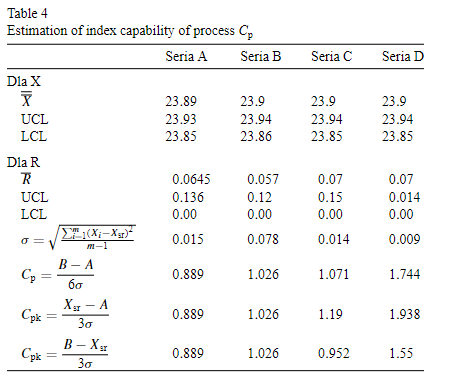
\includegraphics[width=0.85\textwidth]{img/review.png}
  \caption{Indici di capacità di processo} 
  {Fonte: M. Dudek-Burlikowska}
  \label{fig:cp-cpk-review.png}
\end{table}

Con l'avanzare del processo di monitoraggio e controllo di qualità i due indici nell'ultima settimana, ``Seria D'' sono arrivati ad un valore maggiore di 1. 
Questo indica che il processo si è adeguato a soddisfare nel soddisfare le specifiche e che i pezzi prodotti cadono completamente nei limiti di tolleranza. 
\cite{qualityi}


Quindi, l'utilizzo di tecniche statistiche per misurare e migliorare la qualità del processo produttivo, sono d'aiuto nella prevenzione di difetti nel loro successivo rilevamento per migliorare la qualità del prodotto finale.

Si concluse che l'implementazione di tali metodologie statistiche per le aziende polacche sono state efficaci nell'evitare molti difetti di produzione.   
\cite{DUDEKBURLIKOWSKA2005736}


